%\begin{itemize}
%	\setlength\itemsep{1pt}
%	\item Describe the system structure.
%	\item Describe the input to the system.
%	\item Describe the output from the system.
%\end{itemize}

%\subsection{System Architecture}
\begin{figure*}[!ht]
  \centering
    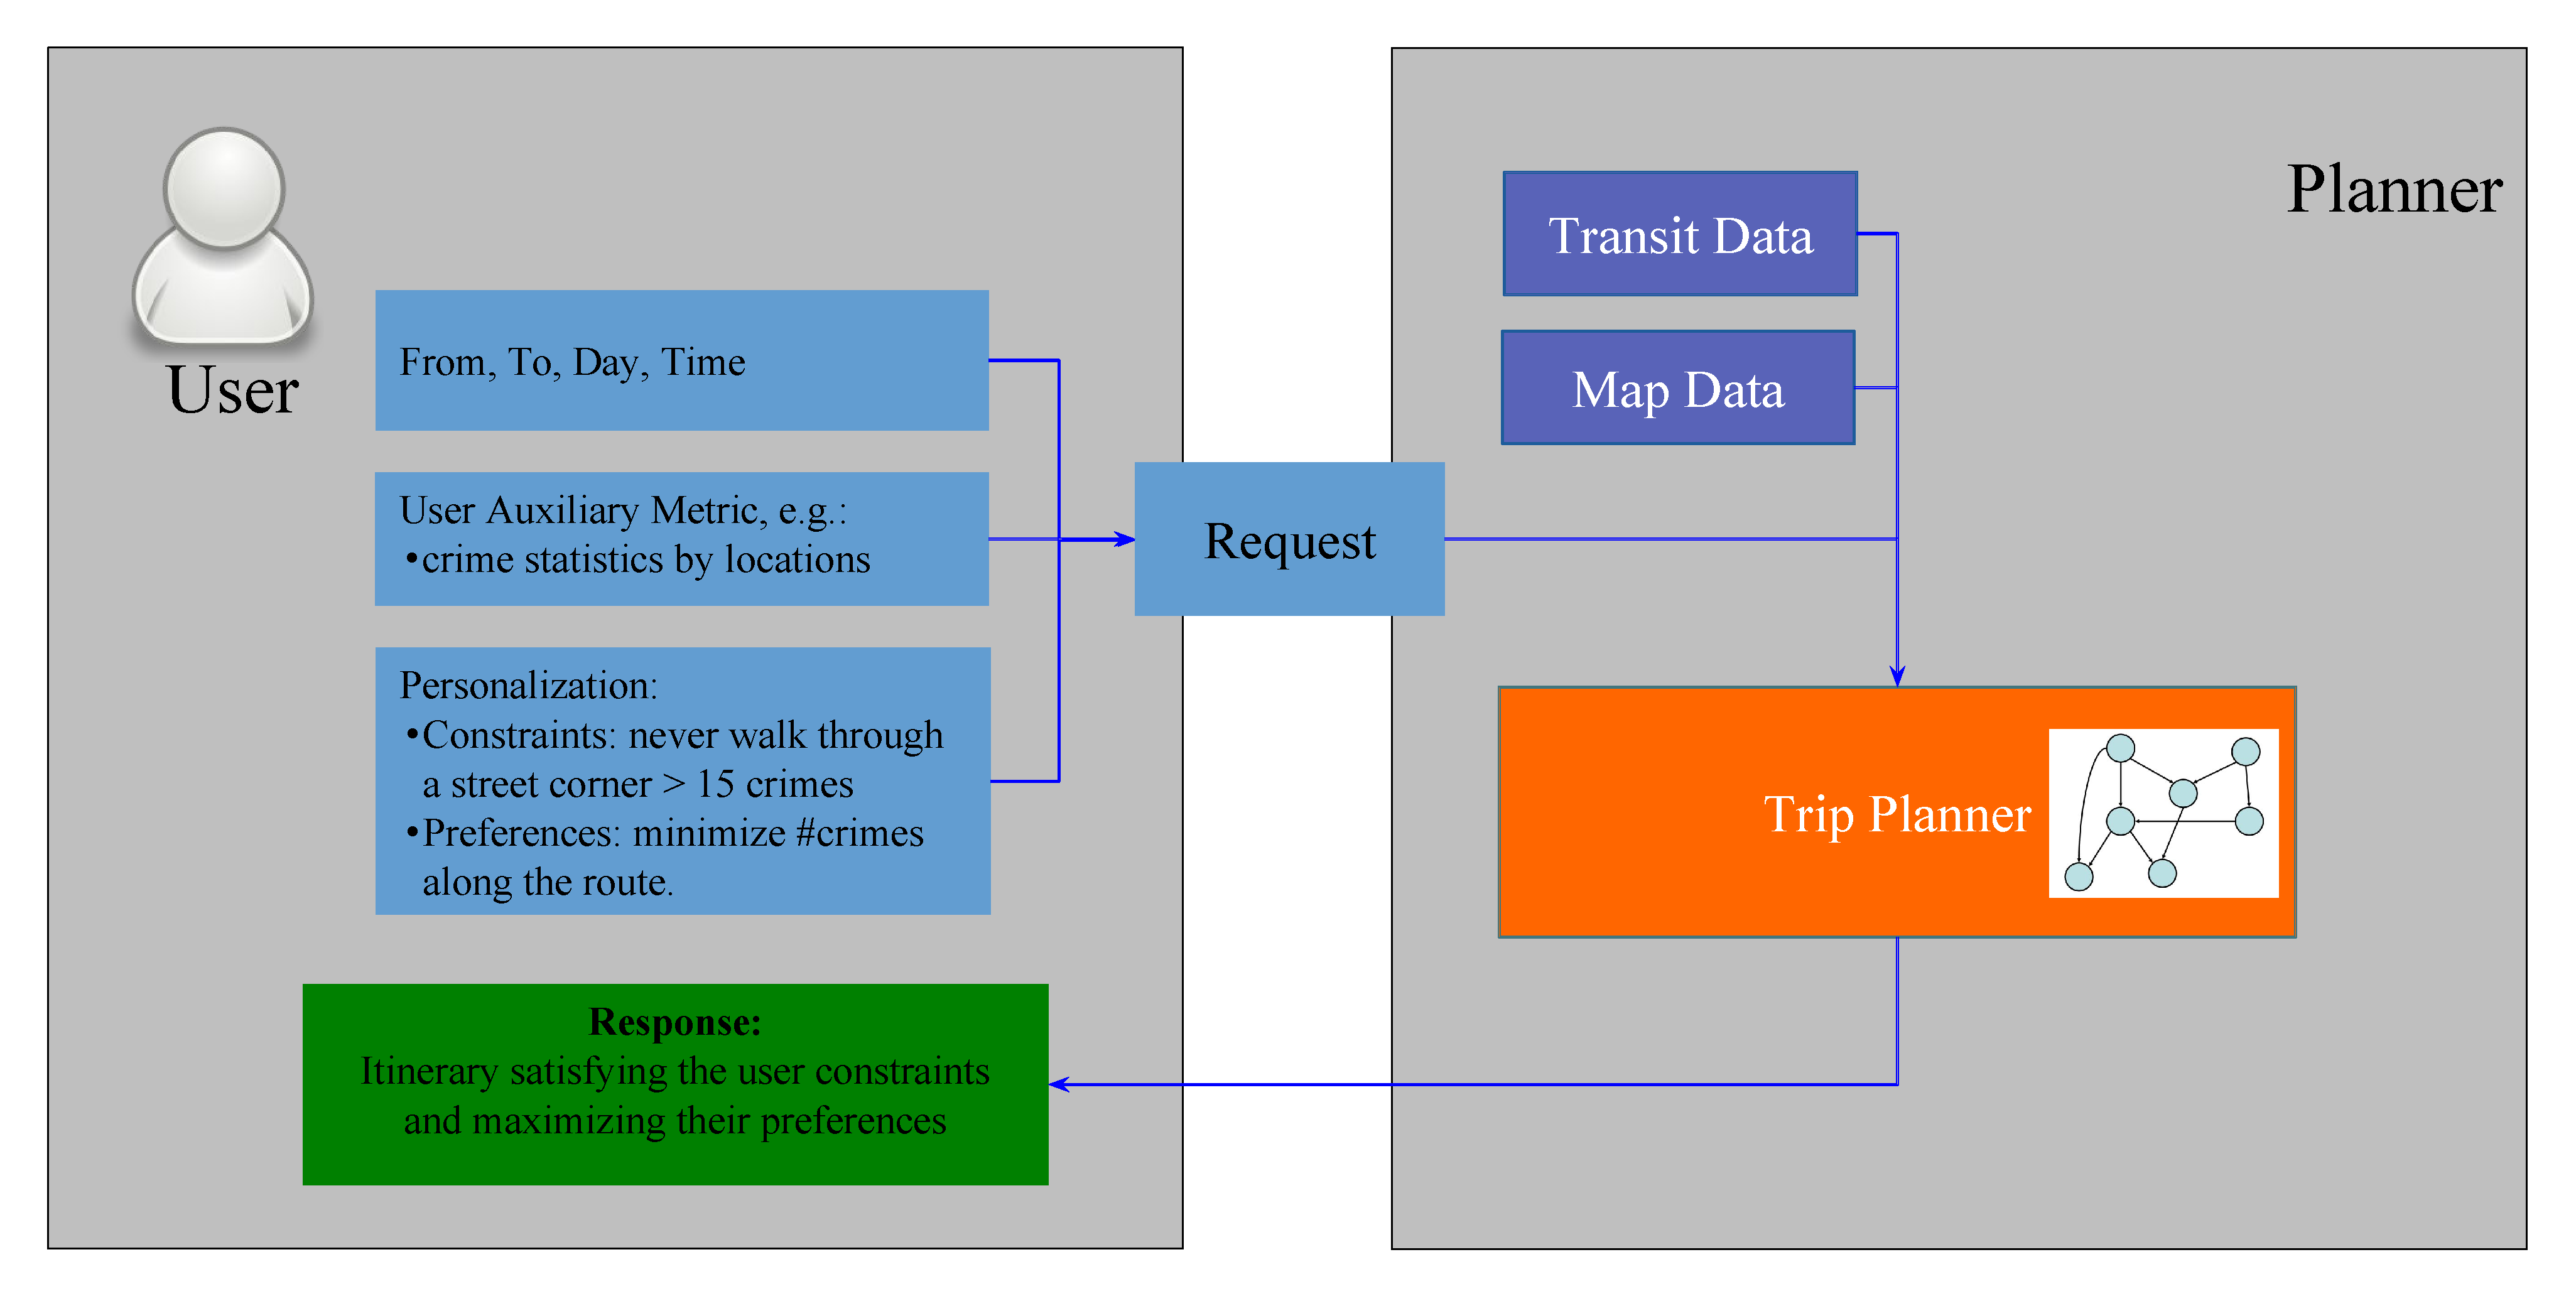
\includegraphics[width=0.8\textwidth]{figs/system.pdf}
  \caption{System Overview\label{fig:system}}
\end{figure*}
We designed and implemented a multi-modal trip planning
system (cf. \figref{system}) based on a 
high-performance graph search engine.
The planner allows user uploads, as well as declarative
constraints and preferences.
We now describe the structure of the planning system.

The trip planner takes two types of data as input:
static data and user-specified request.
The static input includes Map Data and Transit
Data.
Map Data describes the map, a directed graph where 
nodes are street corners, bus stops and train stations.
Transit Data is a set of schedules for the buses and trains
On the other hand, a user provides her request, composed of 
three parts.
First, the user enters \tit{from} and \tit{to} locations 
on the map together with day and time of the start of the trip.  
Second, the user may upload her auxiliary metric dataset, e.g., crime rates.  
Lastly, the user specifies her constraints in LTL and preferences as a $\PCF$.
For example, the constraint 
could be ``never walk through a bad neighborhood."  Given these 
inputs, our planner computes an optimal path satisfying 
all the constraints and optimizing the preferences.
Note that the request from the user is encapsulated into
a JSON object.

For instance, the JSON object for the constraint $\psi$ in \eqtref{ex}
is shown in \figref{exJSON}.
\begin{figure}[!ht]
  \centering
    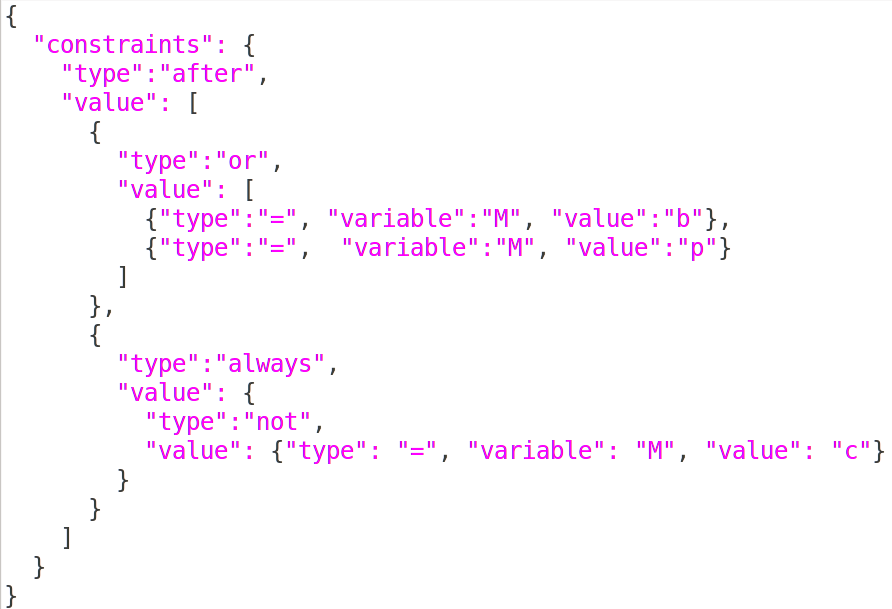
\includegraphics[width=0.5\textwidth]{figs/exampleJSON.png}
  \caption{JSON object for constraint $\psi$ in \eqtref{ex}\label{fig:exJSON}}
\end{figure}
